\documentclass[11pt]{article}
\usepackage[margin=1in]{geometry}
\usepackage{graphicx}
\usepackage{booktabs}
\usepackage{enumitem}
\usepackage{hyperref}
\usepackage{ragged2e}
\usepackage{float}

\title{\textbf{Moved Object Detection with DETR (Option 2: Pixel Diferences)}\\
\large{Computer Vision}}
\author{Hailemariam Mersha (NetID: hbm9834)}
\date{\today}

\begin{document}

\maketitle
\justifying

\section*{\textbf{Overview}}
This report describes my implementation of Option~2, where moved-object detection is performed by feeding a pixel-wise RGB difference of two frames into \texttt{facebook/detr-resnet-50}. The pipeline consumes only the matched annotation text files and produces direct DETR training targets without requiring any intermediate formats. The model predicts bounding boxes on the second frame, corresponding to the final locations of objects that moved. I describe the dataset construction, preprocessing, training setup, ablation results, and visualization outputs.

\section*{\textbf{Method}}

\subsection*{\textbf{Data construction}}
Dataset samples are created using the matched output generated by \texttt{data\_ground\_truth\_labeller.py}. For each pair of frames:

\begin{itemize}[leftmargin=*]
    \item The two frames are loaded at native resolution.
    \item Their absolute pixel-wise RGB difference is computed:
    \[
    \text{diff}(x,y) = |I_2(x,y) - I_1(x,y)|.
    \]
    \item Each annotation file contains two lines of bounding boxes: first-frame boxes and second-frame boxes.
\end{itemize}

Only the second-frame boxes serve as ground truth, since the task is to detect where the object ends up after moving. Extremely small or invalid boxes are filtered. If an annotation contains no boxes after filtering, the sample is skipped. The dataset is shuffled with a fixed seed and split 80/20 into training and validation subsets.

\subsection*{\textbf{Preprocessing}}
All preprocessing is delegated to \texttt{DetrImageProcessor}. It performs resizing using the modern \texttt{shortest\_edge}/\texttt{longest\_edge} interface, normalization using DETR’s ImageNet statistics, and automatic construction of training targets. The custom collate function handles variable-size inputs, preserves metadata for visualization, and excludes invalid samples. Importantly, the entire workflow preserves the spatial consistency required for accurate bounding-box regression.

\subsection*{\textbf{Model}}
The model used is \texttt{facebook/detr-resnet-50}, modified with a six-class detection head for:
\[
\{\text{unknown}, \text{person}, \text{car}, \text{other vehicle}, \text{other object}, \text{bike}\}.
\]

The prediction and bounding-box layers are reinitialized accordingly. Four fine-tuning configurations are supported:
\begin{enumerate}[leftmargin=*]
    \item \textbf{all}: updates the entire DETR model,
    \item \textbf{backbone\_only}: updates only the convolutional backbone,
    \item \textbf{transformer\_only}: updates only the DETR transformer layers,
    \item \textbf{head\_only}: updates only the classifier and box-regressor heads.
\end{enumerate}

\subsection*{\textbf{Training setup}}
Training uses AdamW with:
\begin{itemize}[leftmargin=*]
    \item learning rate $1\times10^{-5}$,
    \item weight decay $1\times10^{-4}$,
    \item batch size 2,
    \item 40 epochs for the baseline,
    \item 100 epochs for each ablation,
    \item gradient clipping (max-norm 1).
\end{itemize}

Validation reports DETR loss, precision, and recall using a score threshold of 0.2 and IoU threshold of 0.5. Only the best checkpoint is retained.

\subsection*{\textbf{Evaluation and visualization}}
The evaluation script computes precision/recall and produces four-panel visualizations showing:
\begin{itemize}[leftmargin=*]
    \item ground-truth boxes (green) on the two input frames,
    \item predicted boxes (red) on the same frames.
\end{itemize}

These visualizations help interpret qualitative behavior such as false positives from shadows or noisy diff regions. Outputs are saved under \texttt{Assignment3/outputs/eval\_vis/} (e.g., \texttt{vis\_000.png} and \texttt{vis\_023.png}).

\section*{\textbf{Results}}

\subsection*{\textbf{Baseline (40 epochs)}}
Training improved recall steadily while precision varied with confidence distribution. The best checkpoint was at epoch 37.

\begin{itemize}[leftmargin=*]
    \item best validation loss: 1.2018
    \item validation precision: 0.302
    \item validation recall: 0.787
\end{itemize}

Validation evaluation yielded:
\[
\text{Precision} = 0.2079,\qquad \text{Recall} = 0.6833.
\]

Although precision is modest, recall remains strong. This behavior is expected with small datasets and a high-capacity model: DETR proposes many candidate boxes, and pixel differences naturally emphasize broader motion regions. Even when inaccurate, these outputs still allow meaningful comparison across fine-tuning strategies.

\subsection*{\textbf{Ablation study}}
The ablations test different fine-tuning scopes and learning rates:

\begin{center}
\begin{tabular}{@{}lcccc@{}}
\toprule
Setting & LR & Validation Loss & Precision & Recall \\
\midrule
all\_lr1e-5 & $1\times10^{-5}$ & 1.0516 & 0.5280 & 0.7580 \\
all\_lr5e-5 & $5\times10^{-5}$ & 1.4008 & 0.2470 & 0.6330 \\
backbone\_lr1e-5 & $1\times10^{-5}$ & 1.8970 & 0.5050 & 0.6210 \\
transformer\_lr1e-5 & $1\times10^{-5}$ & \textbf{1.3291} & \textbf{0.6000} & \textbf{0.7250} \\
head\_lr1e-5 & $1\times10^{-5}$ & 1.4823 & 0.2080 & 0.7040 \\
\bottomrule
\end{tabular}
\end{center}

\subsection*{\textbf{Interpretation of ablations}}
The transformer-only setting delivered the strongest balance of precision (0.60) and recall (0.725), confirming that adapting the attention layers best captures the motion-centric cues in pixel differences. The all\_lr1e-5 run also performed well, while the higher learning-rate variant hurt precision. Backbone-only fine-tuning improved recall but lagged in loss, and the head-only setting pushed recall yet depressed precision, indicating overconfident logits without representational gains. Overall, transformer-only is the safest and most effective scope for this data volume.

\section*{\textbf{Qualitative analysis}}
Visual inspection confirms that pixel differences highlight motion effectively. The model reliably detects moved vehicles and pedestrians, even when frame changes are subtle. Errors typically arise from shadows, lighting variation, or diff noise. The transformer-only variant produces the cleanest boxes and avoids many duplicate predictions.

\section*{\textbf{Design decisions}}
\begin{itemize}[leftmargin=*]
    \item Pixel-wise differences provide a simple yet effective representation of motion.
    \item Using \texttt{DetrImageProcessor} ensures consistent resizing and normalization.
    \item Training directly from the matched text annotations reduces overhead.
    \item Lower score thresholds are appropriate for small datasets, where DETR's confidence calibration differs from large-scale pretraining.
\end{itemize}

\section*{\textbf{Reproducibility}}
Experiments can be reproduced via:
\begin{enumerate}[leftmargin=*]
    \item \texttt{python data\_ground\_truth\_labeller.py}
    \item \texttt{python train.py --strategy all}
    \item \texttt{python eval\_detr\_moved.py --ckpt <path>}
    \item \texttt{python run\_ablations.py}
\end{enumerate}

All outputs are saved under \texttt{Assignment3/outputs/} (see \texttt{outputs/eval\_vis/vis\_000.png} and \texttt{outputs/eval\_vis/vis\_023.png} for examples).

\section*{\textbf{Conclusion}}
The Option~2 approach demonstrates that DETR can detect moved objects using only pixel-wise frame differences. Despite a limited dataset and modest training schedules (40--100 epochs), the ablation study clearly indicates that transformer-layer fine-tuning is the most effective strategy. Pixel-diff DETR offers interpretable visual results and reliably captures motion-related patterns, even when precise localization remains challenging.

\section*{\textbf{Sample outputs}}
\begin{figure}[H]
\centering
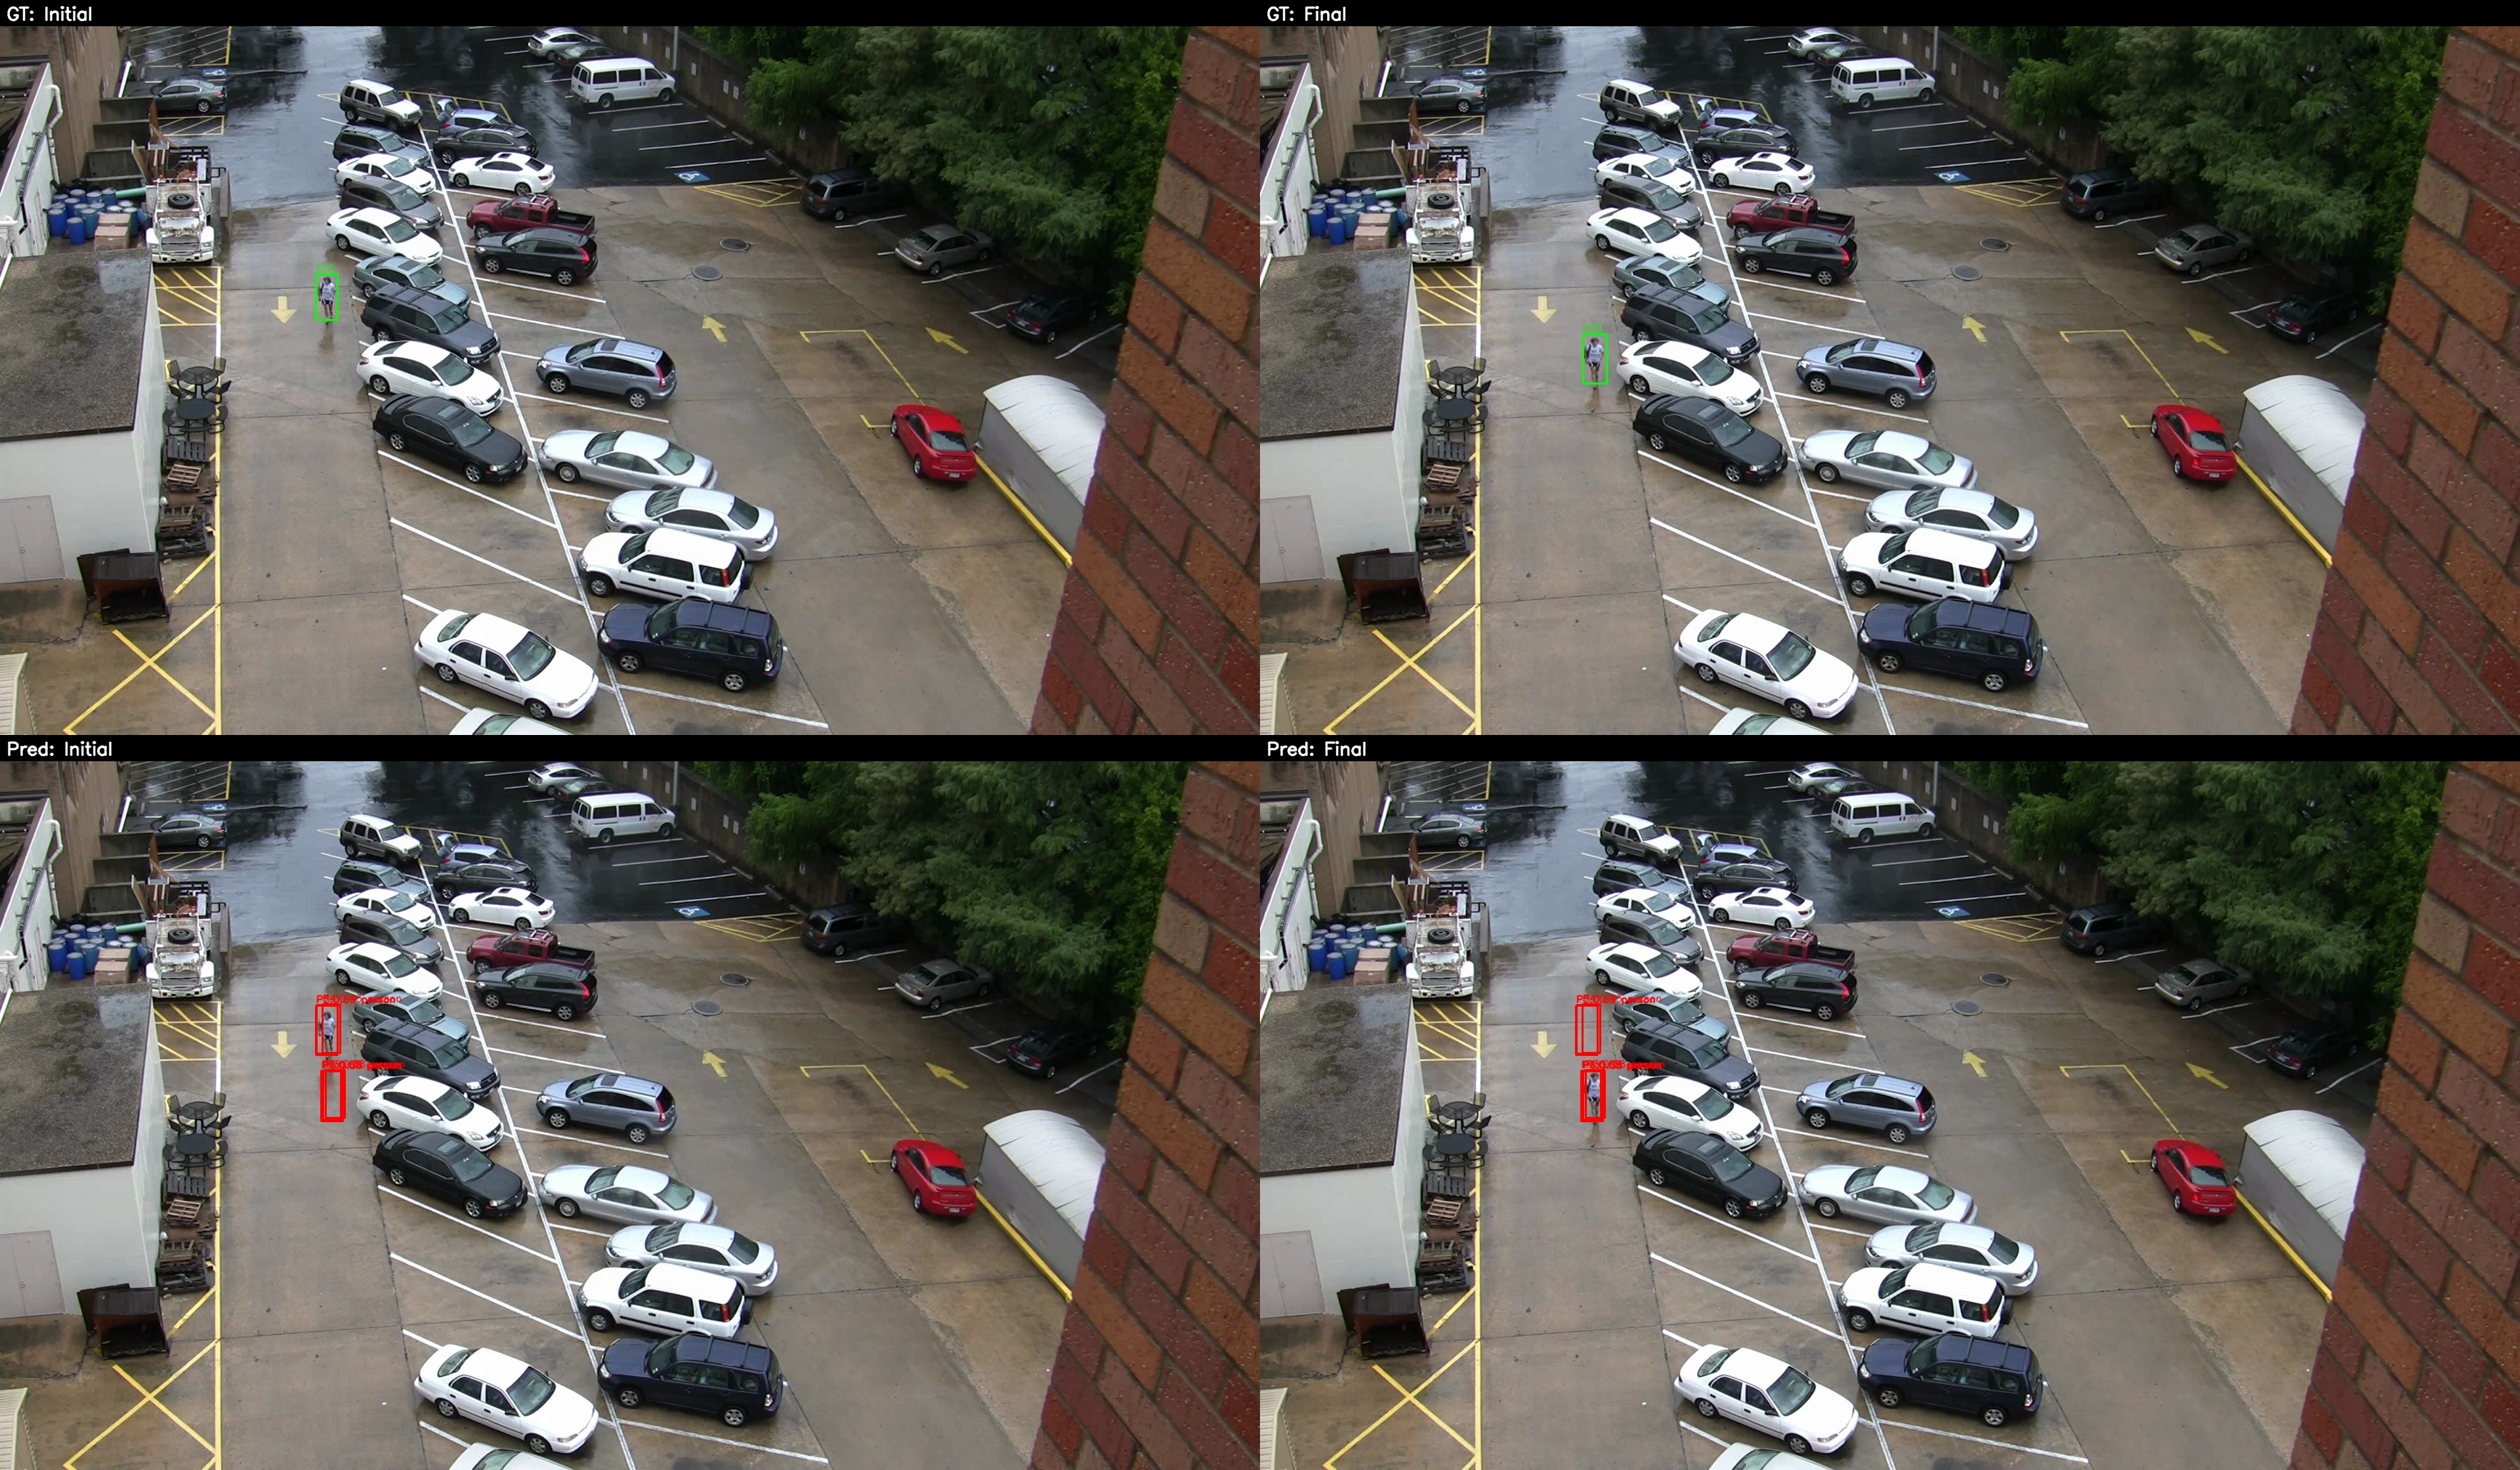
\includegraphics[width=0.9\textwidth]{Assignment3/outputs/eval_vis/vis_000.png}
\caption*{}
\end{figure}

\begin{figure}[H]
\centering
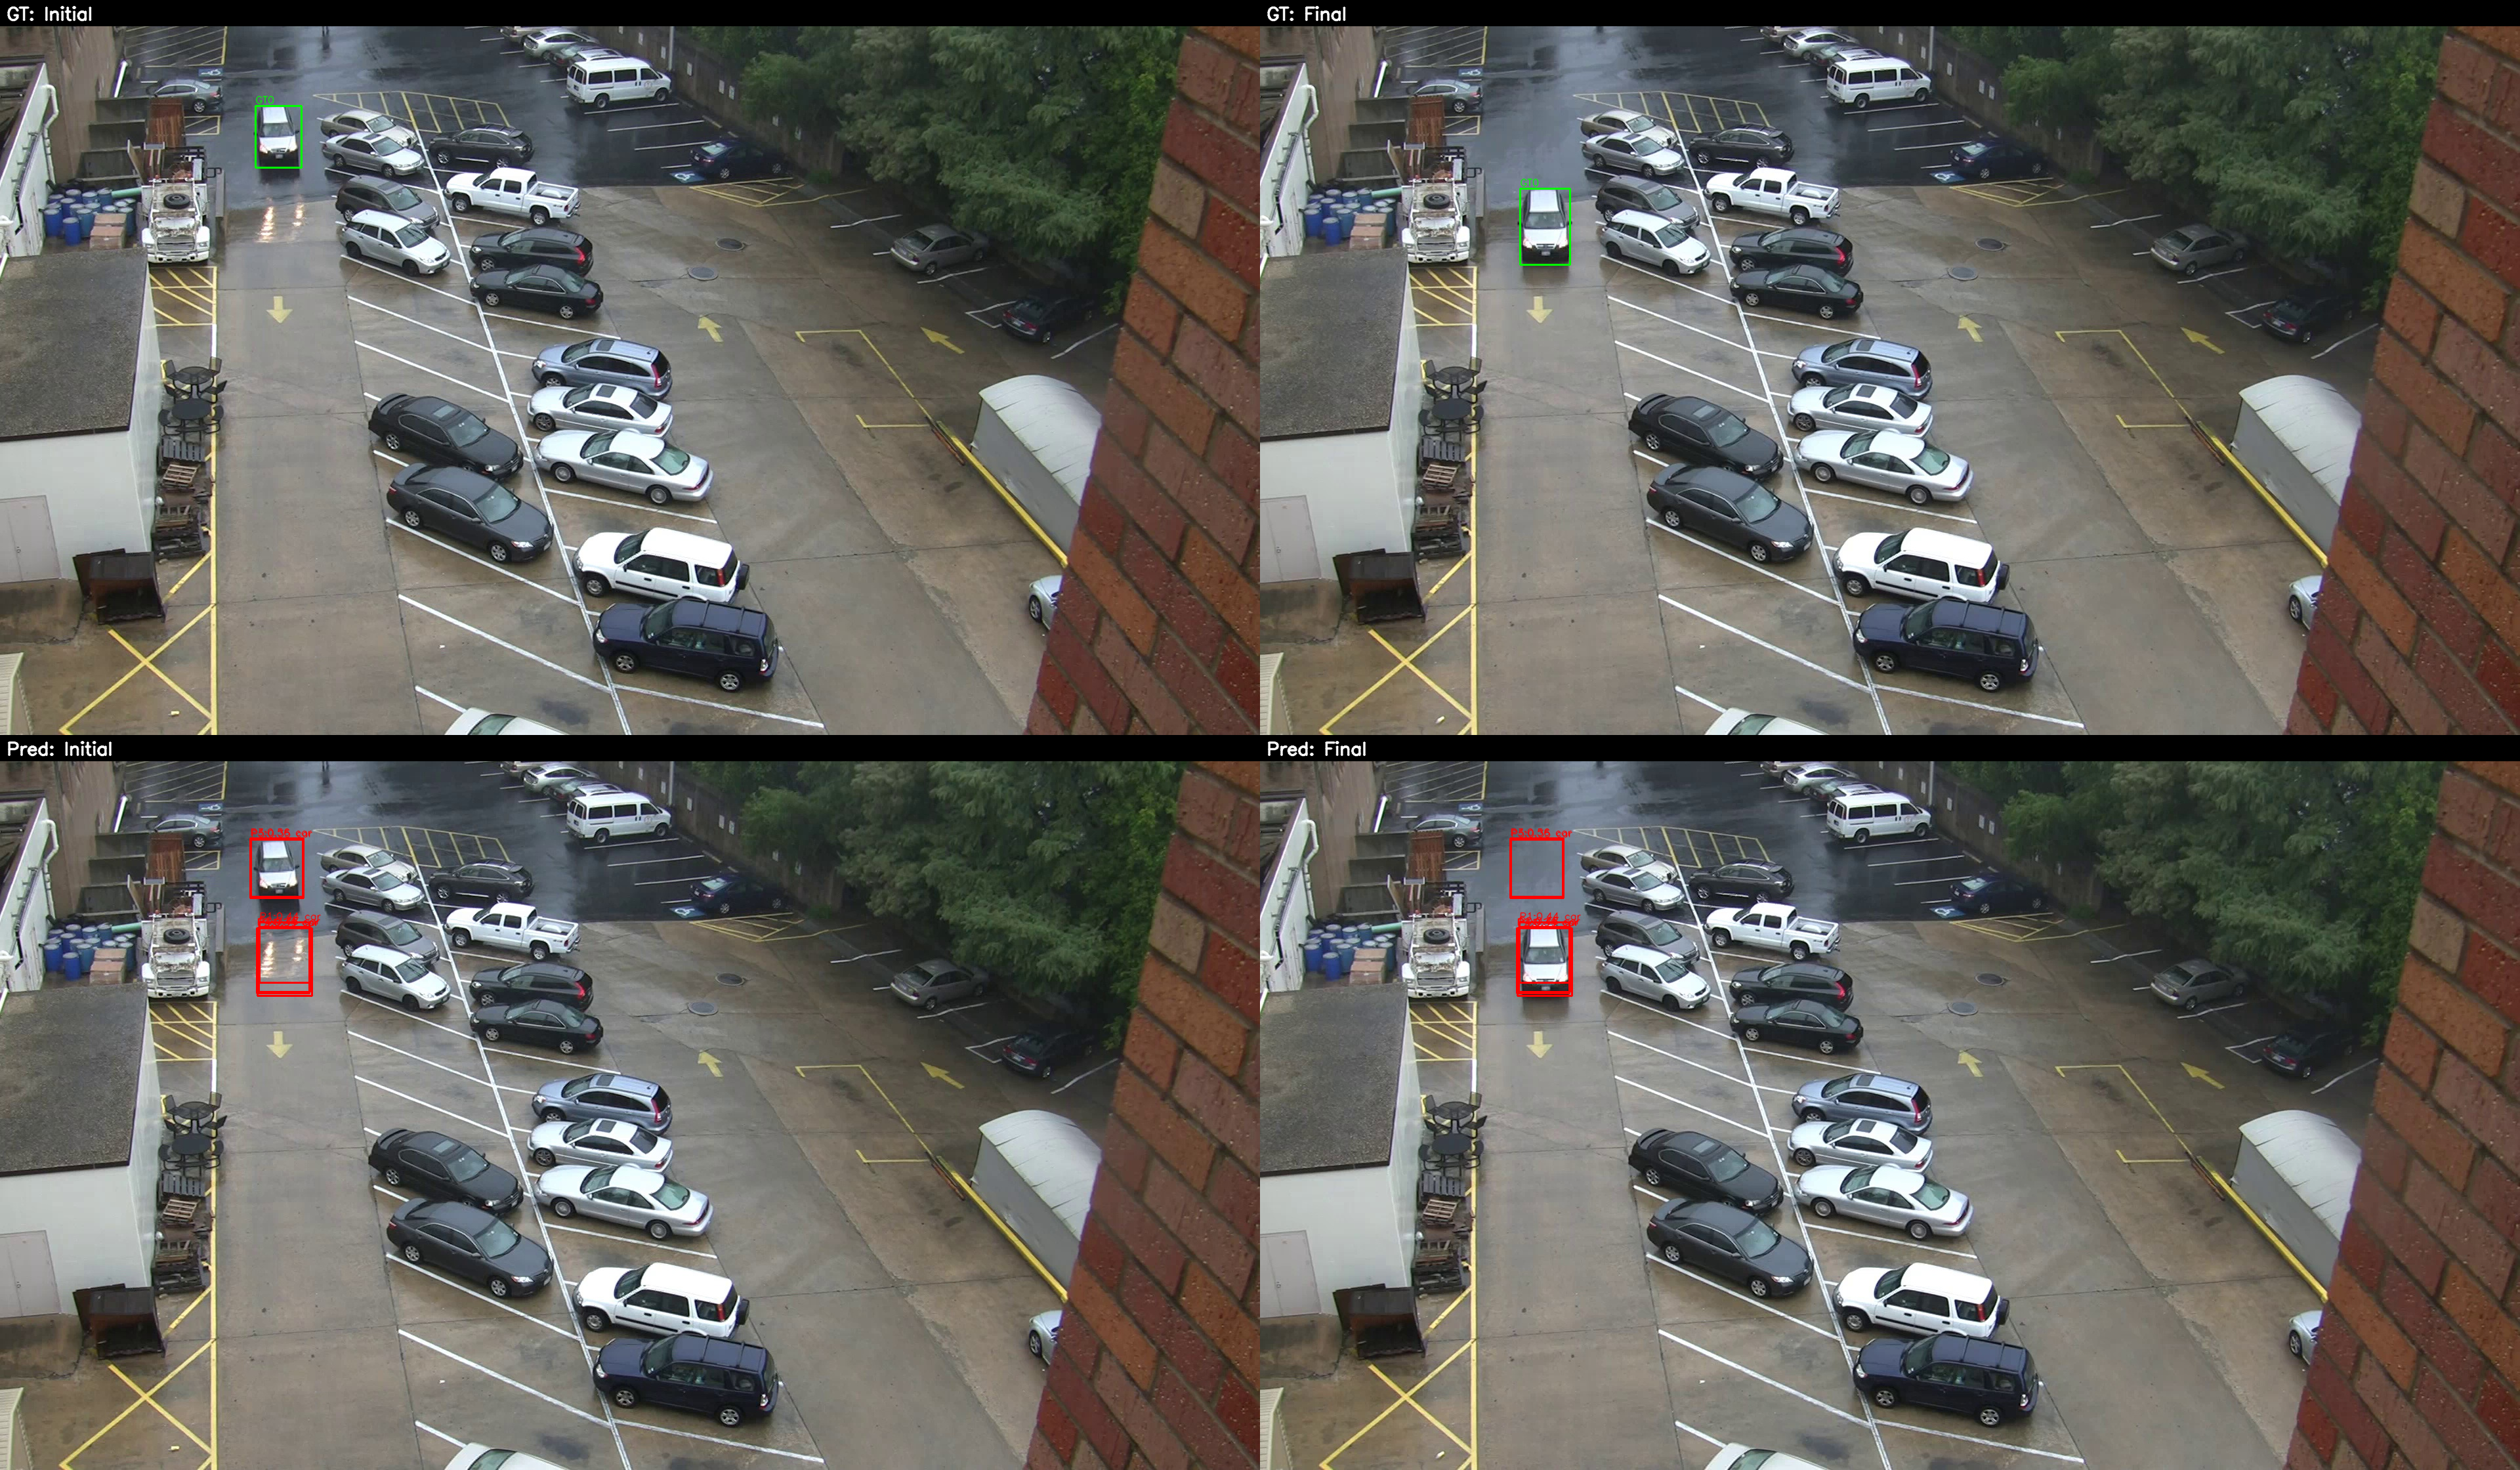
\includegraphics[width=0.9\textwidth]{Assignment3/outputs/eval_vis/vis_023.png}
\caption*{}
\end{figure}

\end{document}
